\documentclass{article}
\usepackage{ctex}
\usepackage{amsmath}
\usepackage{graphicx}
\usepackage{wrapfig}
\usepackage{caption}
\usepackage[top=0.8in, bottom=0.8in,left=0.8in, right=0.8in]{geometry}
\usepackage{float} 
\usepackage{subfigure}
\usepackage{subcaption}
\usepackage{bm}
\xeCJKsetup{CJKmath=true} 

\begin{document}
\section*{虚光子与作用力(40分)}
近代物理认为,粒子之间碰撞时的能量变化是通过交换粒子完成的,本题对此种物理过程作一些简单的计算与分析(\textbf{送分题,不要跳过——SKM})
\begin{itemize}
    \item[(1)] 试就两粒子以任意大小、方向的动量发生碰撞,证明此过程若是为两粒之间传递一个粒子,该粒子的质量不可能为非零实数。(仅就正碰情况下讨论的不得分)
    \item[(2)] 在该类过程中较短时间$\Delta t$内,交换的粒子允许的能量守恒的微小偏离$\Delta E$,若满足Heisenberg不确定关系,即$\Delta E\cdot \Delta t\le\dfrac{\hbar}{2}$此间取$\Delta E\cdot \Delta t\ \~{}\ \hbar$
    \item[(3)] 对于核力,其力程约为$\Delta x\approx 2\mathrm{fm} $该估计核力中交换粒子的静能.
    \item[(4)] 基于此种思想,Y.Yukawa通过核力与电磁力的类比提出核力的介子理论.认为核力的作用是通过交换$\pi$介子完成的,$\pi$介子的存在于12年后得到证实。\par 该例子分为$\pi^0,\pi^+,\pi^-$分别带电$0,e,-e$,质子中子利用其产生作用的方式,如下图\par
    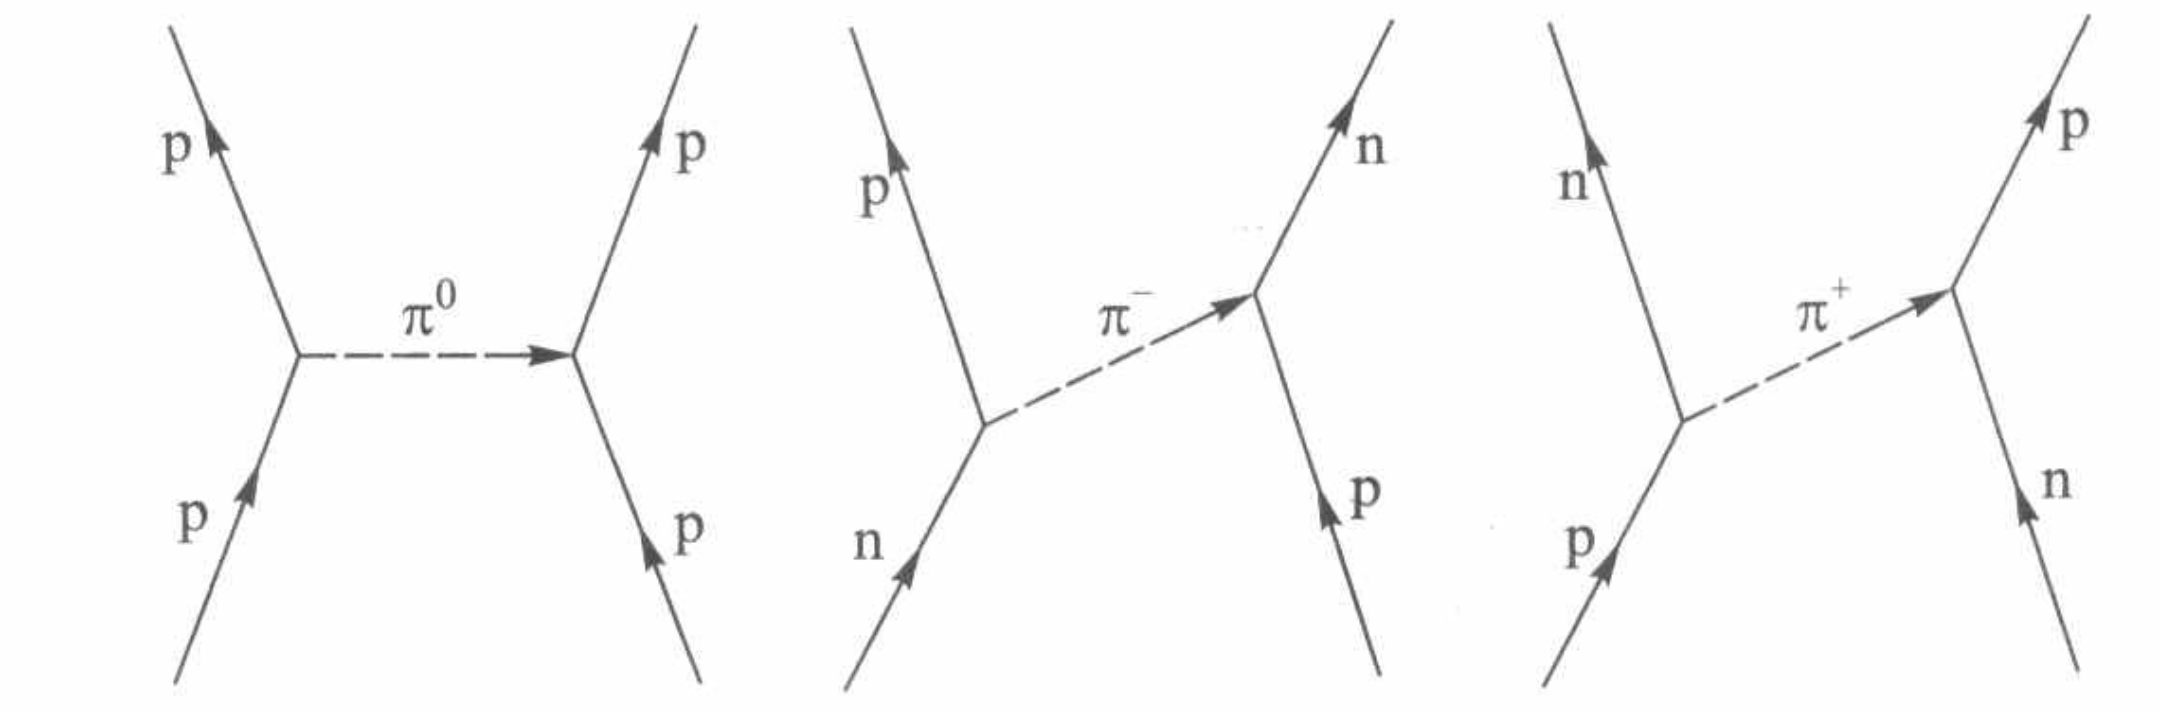
\includegraphics[scale=0.4]{img/0012.1.png}\par
    并在以上过程可保持初末粒子均静止,已知$|m_p-m_n|\ll m_{\pi}$.粒子波函数为复数形式的球面波(与光波相同),是证明$\pi$介子的动量与虚数并给出和相互作用势能(与波函数成正比)与$r$的依赖关系
    \item[(5)] 请回答电磁相互作用中交换粒子是?
\end{itemize}
\end{document} 